%!TEX root = ../Touch Based Idris.tex
\chapter{First Design Iteration}
\label{sec:InitialDesign}

In this section we describe our initial design. 
We designed it based on the findings described in Section~\ref{sec:Analysis} and the requirements derived from these in Section~\ref{sec:GoalsAndRequirements}.
Based on our findings on touch-based editors in Section \ref{subsec:TouchBasedEditors} we are certain that free-text editors rely too much on the virtual keyboard, which provides for a slow work flow and essentially a bad user experience.
We have decided to move towards a more structured editor that makes use of
visual elements to communicate program structure. This approach takes
advantage of the touch platform it is running on instead of trying to overcome
it.

This initial design focuses on the flow of creating function and data declarations. A later iteration (see Section~\ref{sec:third_design_iteration}) will address editing and deleting declarations more throughly.

\section{Overall Structure}
For our initial design we wanted to create a semi-structured editor that lets the user specify data declarations and functions in a structured way, but allows the user to enter free-form text
in terms.
We realized this through a hierarchy of text input fields, that together would make up a data or function definition, somewhat inspired by the structured editing of Lisping.
We also wanted to use visual elements to indicate program structure like we saw in Labview, but as Idris is a general purpose language, the visual elements also have to be more general.
We chose this structured approach as it helps fulfill the following goals and requirements:
\begin{itemize}
	\item \textbf{G-3}: By lifting elements, that would otherwise be text, into the UI itself, we can avoid using the keyboard in many situations.
	\item \textbf{U-1}: The structure of the program can become part of the UI as well. 
	This means we can use special visual cues to differentiate different elements of a program. 
\end{itemize}

% So far: G-3, U-1

One of our takeaways from Lisping was to avoid littering the program text itself with UI elements
(Ta-10).
To help manage this, we adapted the way TouchDevelop manages focus.
When editing a top-level declaration, it should have a special appearance that takes up more space compared to declarations that are not in focus.
This extra space ensures that the elements of the declaration in focus are big enough to be easily tappable. 
Apple recommends that tappable elements are at least 44 points high/wide\,\cite{mobileHIG}, so that has
been our guideline.
At the same time, we can hide unnecessary UI in the declarations that the user is not editing, decreasing clutter.
This focus mode helps the design live up to the following requirements:
\begin{itemize}
	\item \textbf{U-1} and \textbf{U-3}: By minimizing declarations not currently being edited, we improve the scalability of the language, as more of a program can be seen at once, thus providing a better overview.
	\item \textbf{U-6}: Lowers clutter, as UI elements for editing only need to be shown for the declaration currently in focus.
	\item \textbf{F-9}: This directly fulfills this requirement.
\end{itemize}

Based on these decisions, we ended up with a design that indicates a clear hierarchy between elements, shown in Figure
\ref{fig:initial_mockup_design}.

\begin{figure}
	\centering
		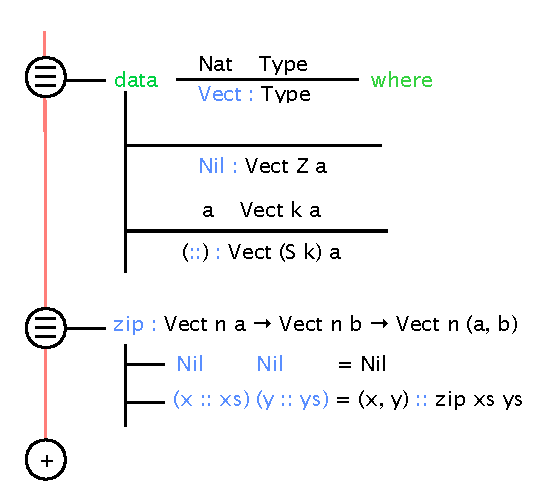
\includegraphics[width=90mm]{diagrams/initial_mockup_design.pdf}
	\caption{Mock-up of a more visual way of representing data types and functions
	in a clear hierarchy.}
\label{fig:initial_mockup_design}
\end{figure}

At the bottom of every construct, there is a round add button, inspired by TouchDevelop, that lets the user add new constructs. These are added to the bottom. 
The round handle buttons connecting each construct to the higher-level vertical line can be used for various code management purposes. 
For example, it is possible to rearrange declarations, clauses, and constructors by dragging these handles. 

Now, if the user wishes to add a new top-level declaration somewhere in the middle of the program, the obvious way would be to use the add button and move the newly created declaration manually. We have, however, designed a faster way.
Reverse-pinching two adjacent handles will create a new declaration between the two existing ones, eliminating the need for rearranging declarations. 
This is a good example of how to use gestures as accelerators for advanced users, and helps us fulfill \textbf{U-4}.
The reverse-pinching gestures is not immediately discoverable (as is the problem with advanced gestures\,\cite[p 141]{nielsen2013mobile}), but power-users will seek faster ways to complete their tasks, for example by reading the accompanying documentation. 
Nielsen and Budiu\,\cite[p 143]{nielsen2013mobile} recommend that you build this sort of redundancy into your app. 
Undo support is implemented as two buttons in the toolbar.
This covers the overall structure of a program in this design. Now we will look at the specifics of declaring functions and data.

% So far: G-3, U-1, U-3, U-4, U-6, F-8, F-9

\section{Function Declarations}
For function declarations we wanted to provide an intuitive flow, using Idris to automate as many steps as possible. 
This meant we had to incorporate initial pattern match creation, case splitting, and automatic metavariable solving into the declaration process.

To be able to declare function types quickly, it was paramount that the interface intelligently presented you with terms that you might have use of.
When a text field takes focus, a context popover with possible terms for that position appears right next to the field. 
The user then only has to move the finger a few centimeters to auto complete the field. 
The usability of this feature depends on how fast and how well the contextual suggestions can be provided.
If the user is looking for a term that is not on the top of the list, it will be necessary to start typing the term manually, until the term list in the context eventually guesses which term is needed. This addresses both \textbf{G-1} and \textbf{G-2}, as well as \textbf{F-7}

% So far: G-1, G-2, G-3, U-1, U-3, U-4, U-6, F-7, F-8, F-9

We did not want to clutter the interface with [+] buttons like Lisping does, so one of the early problems that we needed to solve was to elegantly indicate where new terms could be added.
We came up with the solution seen in Figure \ref{fig:initial_function_editing_design}.
When the user starts typing in the rightmost empty text field, a new text field pops up to indicate that further terms can be added to the type declaration. This is in compliance with \textbf{U-6}.

\begin{figure}
	\centering
		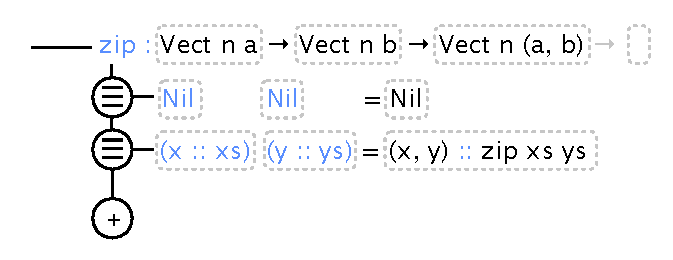
\includegraphics[width=110mm]{diagrams/initial_function_editing_design.pdf}
	\caption{Mock-up of a function in edit mode. Notice the indication that expressions can be
	added at the rightmost end of each line.}
\label{fig:initial_function_editing_design}
\end{figure}

Pressing the plus button on a function with no clauses will add a clause with an initial pattern, with the pattern variables named intelligently. 
Double tapping a pattern variable will perform a case split if possible. 
The use of this gesture is also a non-standard one, and a tip will have to appear one of the first times case splitting is possible.

Finally, metavariables, expressed as three question marks, can be tapped for automatic metavariable solving. 
There should be clear feedback to the user regardless of the outcome of this action.

Together these features leverage the tool support afforded by Idris to fulfill \textbf{F-1}, \textbf{F-2}, \textbf{F-3}, as well as partially fulfilling \textbf{F-5}. To fully fulfill \textbf{F-5}, we must also support deleting functions, as well as cases. This will be addressed in
Section\,\ref{sec:third_design_iteration}. \todo{make sure we describe this}

% So far: G-1, G-2, G-3, U-1, U-3, U-4, U-6, F-1, F-2, F-3, F-7, F-8, F-9

\section{Data Declarations}
Instead of staying visually close to textual Idris, as we had done with function declarations, we decided to try an alternative approach for data declarations, inspired by Epigram.
This resulted in a more visual way of representing data definitions, where a data definition looks less like a function, and more like a logical inference rule.
Any parameters for the type are written as premises (above the horizontal line), with the type being the conclusion
(below the line to the right of the colon). The type identifier is written
below the horizontal line to the left of the colon.
Constructors are written in the same manner, with arguments as premises, and the constructed type as the conclusion.
Our hope was that this way of declaring data would be more visually appealing, while still enabling a smooth work flow, in accordance with \textbf{U-1}.
The premises of the type constructor and subsequent constructors use the same flow of input as the type declaration of functions.
The reuse of the flow allows the user to learn its behavior once and then use it with a certain feeling of familiarity in the rest of the UI\@.

\begin{figure}
	\centering
		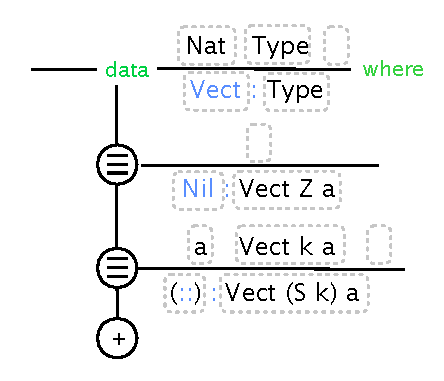
\includegraphics[width=80mm]{diagrams/initial_data_declaration_design.pdf}
	\caption{Mock-up of a data declaration design in edit mode. The syntax
	resembles the 2D Epigram syntax}
\label{fig:initial_data_declaration_design}
\end{figure}

\section{First Usability Iteration}
\label{sec:UsabilityTest}
With a design in hand, it was time to test it. The purpose of this test was to
get an initial idea of how our ideas worked before spending time implementing
them. We created paper cutouts based on our mock-ups to represent the different
elements of the interface, with a test facilitator manipulating the cutouts to
emulate an interactive environment. The procedure of the experiment was inspired by Chapter 10 of ``Observing the user experience''\cite{kuniavsky2003observing} and a more detailed test report is available in Appendix \ref{chap:FirstUsabilityTest}. The report includes a timestamped summary of the test, which we
will sometimes refer to in the following manner: S1.1, which refers to the
first point in the summary for subject \#1.

\subsection{Participants}
As it is beyond the scope of this project to teach new users about dependent
types, our test participants needed experience with a programming language
featuring dependent types, ideally Idris, prior to our test. This obviously
severely limited the number of readily available candidates. Because we wanted
to conduct later tests with subjects without knowledge of earlier iterations of
the design, we limited ourselves to two test subjects for this first test. An
overview of the test subjects can be see in Table~\ref{table:first_test_subjects}.

\begin{table}
\centering
\begin{tabular}{| l | l | p{5cm} | p{5cm} |}
\hline
Subject & Age & Occupation & Experience \\ \hline
\#1 & 24 & Masters student at IT-University studying programming languages & 6 months experience with Idris, several years of experience with functional languages in general \\ \hline
\#2 & 27 & Masters student at IT-University studying programming languages & 6 months experience with Idris, several years of experience with functional languages in general \\ \hline
\end{tabular}
\caption{Test subjects}
\label{table:first_test_subjects}
\end{table}

\subsection{Session Details}
The test was conducted in a meeting room at the IT University, with three
people present: The test subject, the test facilitator, and a note taker. The
tests were recorded. First, the test subjects were told about the project in
general. They were then told of the overall structure of the test: They would
be given two tasks, with three steps each. Each step would be explained when
they reached it. They were asked to think aloud during the test, and were told to
ask if they felt they had been stuck for a long time. Periodically, we would
ask questions about what they were thinking. At the end of the test, they were asked for general feedback on the test.

\subsection{Tasks}
The two tasks they were asked to complete are listed in Figure~\ref{figure:first_tasks}.
It should be noted that since the test was concerning the interface itself, and
not programming in Idris, the test subjects had access to the definitions for \texttt{Vect} and \texttt{zip} in textual Idris. Refer to Section~\ref{subsec:Idris}
for more on \texttt{Vect} and \texttt{zip}.

\begin{figure}
\centering
\begin{itemize}
	\item \textbf{Task 1}: Define a data declaration for the vector type.
	\begin{itemize}
		\item \textbf{T1.1}: Specify an identifier for the type (\texttt{Vect}), along with its type (\texttt{Nat -> Type -> Type})
		\item \textbf{T1.2}: Specify the Nil constructor (\texttt{Nil: Vect z a})
		\item \textbf{T1.3}: Specify the Cons constructor (\texttt{(::): a -> Vect k a -> Vect (S k) a})
	\end{itemize}
	\item \textbf{Task 2}: Define the zip function for vector type.
	\begin{itemize}
		\item \textbf{T2.1}: Specify the identifier for the function (\texttt{zip}), along with its type (\texttt{Vect k a -> Vect k b -> Vect k (a, b)})
		\item \textbf{T2.2}: Specify the first case (\texttt{zip Nil Nil = Nil})
		\item \textbf{T2.3}: Specify the second case (\texttt{zip x::xs y::s = (x, y) :: zip xs ys})
	\end{itemize}
\end{itemize}
\caption{Tasks for the first usability. The text in parentheses are what we considered the correct answer, and was not given to the test subjects.}
\label{figure:first_tasks}
\end{figure}

\subsection{Issues}
\label{sec:first_issues}
As was expected, several issues were encountered. It was quickly apparent that
the data declarations were the most problematic aspect of the design, and that
we would need to revisit their design. Task 2 on the other hand went quite
smoothly in comparison, and both subjects were impressed by the degree to
which Idris could save them from typing. We have listed the issues we
encountered below. \\ \\
\textbf{I1: Data declarations}.
The main issues our test subjects experienced had to do with the data
declarations. While both subjects had seen this way of writing types
before, it was not immediately clear to them how they should be filled out.
They did eventually get through it, but they required a great deal of help
from the test facilitator. Especially step T1.1 was difficult. (S1.1--8, S2.4, S2.9--15)\\ \\
\textbf{I2: Suggestions for parameterized types}.
When filling in a type, a contextual popover with suggestions would appear. In our mock-up,
these suggestions were always correct. But both subjects wondered how one would
fill in types that take multiple parameters. (S2.29) \\ \\
\textbf{I3: Gesture overload}
One subject wondered how to differentiate gestures for editing versus
gestures for case splitting or autocompletion. For example, double tapping on
text already has an action associated with it. (S2.34) \\ \\
\textbf{I4: Managing contexts}
After having finished step T1.3, both subjects had trouble leaving the editing
context. Only after a great deal of experimentation did they manage to leave
it. Both subjects tried to use the undo and redo buttons to change contexts.
(S1.10--13, S2.21--23)

\subsection{Recommendations}
\label{sec:first_recommendations}
Since issue \textbf{I1} was by far the most problematic issue we discovered, we have
focused on mitigating it in our recommendations. The basic strategy is to make
it easier to understand through examples and help in the interface. If the
changes listed below are not enough, it might be necessary to completely
redesign the data declarations, perhaps by modeling them more closely after how
they look in textual Idris.

\begin{itemize}
	\item \textbf{Re1} (I1): In the text field for inputting the name and type for Data, insert an initial colon (``\texttt{:}''), separating the identifier from the type. This might make it easier to see what goes where.
	\item \textbf{Re2} (I1): Have initial hint text in text input fields, in a light color, which disappears when the fields gain focus. E.g. in the text field for the identifier, it could say ``Identifier'' or ``Name'', while the input field for the type can say ``Type''.
	\item \textbf{Re3} (I1): Differentiate borders around text fields more, to make it clear which fields have been filled, which must be filled, and which might be filled.
	\item \textbf{Re4} (I1): Show the definition for \texttt{Nat} to begin with, so the user can see an example.
	\item \textbf{Re5} (I2): Do not try to fill parameters for types, as we cannot know what they will be. Instead, just leave blank spaces so the user can fill them in.
	\item \textbf{Re6} (I3): To avoid conflict between editing and case splitting/autocompleting, implement a new gesture for ``auto'', perhaps swiping down on a term.
	\item \textbf{Re7} (I4): Implement a button or other UI element that designates the declaration is done. This could be in the form of a check mark, or some other symbol.
\end{itemize}

% So far: G-1, G-2, G-3, U-1, U-3, U-4, U-6, F-1, F-2, F-3, F-7, F-8, F-9

\section{Design Evaluation}
\label{subsec:first_design_evaluation}
While this initial design meets many of the requirements from Section~\ref{sec:GoalsAndRequirements}, there are still issues to resolve.
Specifically, the following requirements are not fully addressed:
\begin{itemize}
	\item \textbf{U-5}: This requires some way to communicate with Idris. The backend required to do this will be covered in Section~\ref{sec:Architecture}, while the design considerations will be covered in
	Section \ref{sec:third_design_iteration}.
	\item \textbf{F-4} and \textbf{F-5}: We have described how to create functions and data declarations, and how one can add and edit clauses and constructors. However, we still need to devise a way to delete these constructs. This will be covered in Section \ref{sec:third_design_iteration}.
	\item \textbf{F-6}: This will be addressed in the next section.
	\item \textbf{F-10}: This will be addressed in Section \ref{sec:third_design_iteration}.
\end{itemize}

Beyond these requirements, the greatest remaining challenge is the data declaration syntax, which we will try to improve in the next design iteration, described in Section~\ref{sec:Implementation}.
We have learned a great deal from this initial design, based on mock-ups and paper cutouts, but for our next iteration, we want to produce a simple prototype app.
Actually implementing our next design will surely uncover many problems not discovered in our mock-ups.
But before we can do this, we need to lay some technical groundwork, which is desicribed in the next section.